
\documentclass[preprint,12pt]{elsarticle}

\usepackage[spanish]{babel}
\usepackage{amssymb}
\usepackage{graphicx}
\usepackage{lineno}
\usepackage[utf8]{inputenc}
\usepackage{url}
\usepackage{natbib}

\begin{document}
	
	\begin{center}
		\huge \textbf{METODOLOGIA INMON VS METODOLOGIA KIMBALL} 
	\end{center}
	\vspace{\baselineskip}
	\begin{center}
		
\includegraphics[scale=0.37]{./IMAGENES/logo}
	\end{center}
	\begin{multicols}

		\begin{center}
		    Villegas Arando, Marlon Xavier\\            2015053890\\
			\columnbreak
			Espinoza Caso, Lisbeth Isabel \\
			2011040667\\               
			
		\end{center}
		\normalsize			
	\end{multicols}
\newpage
	\begin{frontmatter}
		\begin{abstract}
The development of a data warehouse is not an easy task, to carry out its implementation it is necessary to have the appropriate methodology; It requires the design of a conceptual model that includes both the information requirements of the users as well as the operational data sources, from which a logical model is obtained based on a specific database technology that guides the implementation. Currently, many of the existing methodologies do not define mechanisms that cover the particular characteristics of the development of a data warehouse, making it a complex and artisanal task. To solve this problem, in this article a study is made of two methodologies for the development of data warehouses, making an analysis of its main characteristics to determine the most appropriate.

		\end{abstract}
\end{frontmatter}

	\section{Resumen}
El desarrollo de un almacén de datos no es tarea fácil, para llevar a cabo su implementación es necesario disponer de la metodología adecuada; se requiere el diseño de un modelo conceptual que incluye tanto los requisitos de información de los usuarios así como las fuentes de datos operacionales, a partir del cual se obtiene un modelo lógico basado en una tecnología de base de datos específica que guía la implementación. Actualmente muchas de las metodologías existentes no definen mecanismos que abarquen las características particulares del desarrollo de un almacén de datos, convirtiéndolo en una tarea compleja y artesanal. Para dar solución a este problema, en este articulo se realiza un estudio de dos metodologías para el desarrollo de almacenes de datos, realizando un análisis de sus principales características para determinar la más apropiada.

\section{Introduccion}
Actualmente las organizaciones utilizan la información y el conocimiento para apoyar la toma de sus decisiones estratégicas, y de este modo lograr sus metas y mejorar sus procesos.
Uno de los desafíos que enfrentan hoy las organizaciones, es el aumento de datos, lo que ha generado dos grandes problemas; el primero, identificar los datos relevantes para dar seguimiento a su estrategia organizacional, y lograr que se cumplan los planes con las metas establecidas. Y el segundo problema, la capacidad para administrar esta gran cantidad de datos.
Un almacén de datos (data warehouse, DW) según Inmon, es una colección de datos orientada a un determinado ámbito (empresa, organización, etc.), integrado, no volatil y variable en el tiempo, que ayuda a la toma de decisiones en la entidad en la que se utiliza. Se trata, sobre todo, de un historial completo de la organización, mas alla de la informacion transaccional y operacional, almacenado en una base de datos diseñada para favorecer el análisis y la divulgación eficiente de datos (especialmente con herramientas OLAP, de procesamiento analítico en línea). Por otra parte Kimball la define como una copia de los datos transaccionales estructurados específicamente para consultas y análisis. 
Las herramientas de BI en la actualidad, son de mucha importancia para la toma de decisiones en las organizaciones, por no interpretar correctamente la información, se generan pérdidas considerables y efectividad en el rumbo de las estrategias a implementar.

En este breve artículo intentaremos brindar una explicación general de dos de las metodologías más usadas, la metodología de Kimball y metodología Inmon.

\section{Objetivo}
		\begin{itemize}
		\item Objetivo 1: Dar una visión clara de BI, desde las perspectivas de los autores que sentaron las bases que son Ralph Kimball y Bill Inmon, para la mejora de las estrategias del negocio al que se desee implementar las herramientas de BI.
		\item Objetivo 2: Describir las metodologías propuestas por los principales autores de BI desde las perspectivas de sus creadores Ralph Kimball y Bill Inmon.
		\item Objetivo 3: Comparar las propuestas hechas por los autores con el propósito de hacer una valoración de las ventajas, desventajas y puntos de su implementación.
		\item Objetivo 4: Identificar aspectos relevantes en las arquitecturas y ciclo de vida de los sistemas DW/BI de ambos autores.
		\item Objetivo 5: Realizar una comparación de la tendencia actual que ha tomado la BI con las propuestas investigadas y generar recomendaciones sobre los procesos de adopción de una metodología. 


	\end{itemize}

\section{Marco Teorico}
	
\subsection{METODOLOGIA SEGUN INMON}	

	Según Bill Inmon, propone que un DW es el conjunto de datos orientados a temas específicos de la organizaciones, es decir deberán ir cambiando con el transcurso del tiempo, pero dichos datos, no deben ser volátiles (no es posible eliminar, ni modificar la información).
Al momento de generar un cambio en los datos, se debe de efectuar de una manera que, quede reflejado el cambio que se efectuó y mantener siempre la integridad de la información, se espera que todo resultado del proceso y transformación de la información por medio de herramientas de BI, sea un firme apoyo para los tomadores de decisiones al momento de orientar una estrategia de negocio.

Bill Inmon, considera que debido al exceso y sobrecarga de información que se está manejando en un DW, estas bases de datos deben estar aisladas y solo manipularse para procesos de BI. Toda información que se almacena en un DW o DM deberá ser
procesada y normalizada antes. La recomendación sobre la información, deberá estar a su máximo detalle posible, con lo cual se logre cubrir todas las necesidades de cada departamento, la importancia a la necesidad de transferir la información de los diferentes OLTP (Sistemas Transaccionales) de las organizaciones a un lugar centralizado donde los datos sean utilizados para el análisis.

Consta de las siguientes características::
\begin{itemize}
		\item Orientado a temas: Los datos en la base de datos están estructurados de forma que los datos estén relacionados.
		\item Integrado: La base de datos contiene todos los datos de los sistemas operacionales de la organización(9), con la característica de ser consistentes.
		\item No volátil: Los datos no se modifica ni se elimina, almacenado los datos, éste se convierte en información de sólo lectura.
		\item Variante en el tiempo: Los datos que sufren un cambio a través del tiempo, deben ser registrados para que los informes generados reflejen esas variaciones.
\end{itemize}

La metodología que Bill Inmon propone es iterativa la cual sigue un esquema contrario al clásico de desarrollo de sistemas ya que lo primero con lo que se trabaja son datos, estos se
integran para ser probados y programar de acuerdo a ellos para analizar los resultados y de esta manera comprender los requerimientos. La metodología principalmente consiste en lo
siguiente:
\begin{figure}[htb]
				\begin{center}
					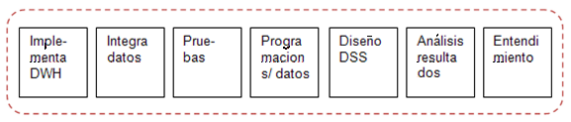
\includegraphics[width=15cm]{./IMAGENES/imgmire1}
				\end{center}
			\end{figure}

Dentro de esta metodología se menciona que la construcción de toda la arquitectura de un Data Warehouse toma bastante tiempo, puesto que su desarrollo inicial está relacionado con
necesidades genéricas empresariales, a lo largo del tiempo este tipo de necesidades son cubiertas por el Data Warehouse para mas personas por lo que la demanda del uso del Data
Warehouse aumenta y esto hace que el performance se vea afectado. Es por esto que al llegar a este punto se comienzan a construir segmentos del Data Warehouse que se alimentaran del
Data Warehouse y que permitirán tener la información almacenada de manera que esta vaya dirigida a departamentos, con esto se logra disminuir la demanda sobre el Data Warehouse
debido a que por ejemplo para estos momento en lugar de tener a 100 usuarios requiriendo de manera directa los servicios del Data Warehouse tendré 5 departamentos.

\begin{figure}[htb]
			\begin{center}
					
\includegraphics[width=15cm]{./IMAGENES/imgmire2}
				\end{center}
			\end{figure}

\subsection{IMPLEMENTACIONES DE  INMON}
1. Implementación del Data Warehouse.
	a. OLTP. El primer paso para la implementación de un Data Warehouse es el identificar las fuentes de datos, analizarlas y mapear sus elementos de acuerdo al estándar que hayamos definido. Esto en el orden de tratar de homologar los datos que sea posible para su entrada al Data Warehouse.
	b. Modelos de Procesos. Se debe tener conocimiento de los procesos que sigue la información y para eso nos sirve el modelo de procesos. Este modelo contiene información como:
\begin{itemize}
	\item Descomposición funcional
	\item Diagrama de contexto
	\item Diagrama de flujo de datos
	\item Diagrama de transición de estados
	\item Pseudocódigo
\end{itemize}

	c. Modelo de datos. Se trabaja con 2 tipos de modelos:
		\begin{itemize}
			\item El Modelo de datos nos muestra los datos primitivos, tomando en cuenta el elemento tiempo, se plasman los cálculos que se realicen y finalmente se muestran sus relaciones.
		\end{itemize}


El Modelo de Datos del Data Warehouse. Los modelos anteriores nos deberán entregar la definición de los sujetos a los que estará orientado el Data Warehouse. Debe venir en 3 perspectivas y son explicadas en la siguiente tabla:
\begin{figure}[htb]

			\begin{center}
					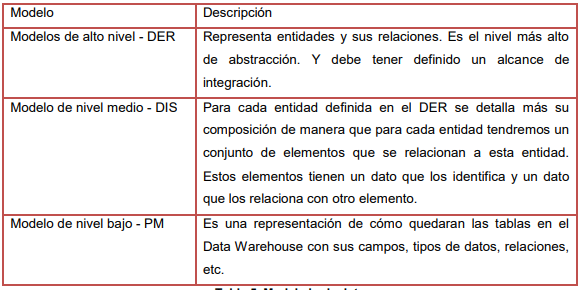
\includegraphics[width=15cm]{./IMAGENES/imgmire3}
				\end{center}
			\end{figure}

	d. Una vez que se tiene conocimiento de este modelo se deben tomar ciertas decisiones sobre el diseño del Data Warehouse. Entre estas decisiones tenemos las siguientes:
		\begin{itemize}
			\item Normalización, debemos decidir el grado al que nuestro Data Warehouse
			\item Granularidad
			\item Particiones
			\item  Minería de Datos
		\end{itemize}

	e. Al haber tomado estas decisiones, se debe generar un documento que contenga estas decisiones que hemos tomado para la definición del Data Warehouse. Este documento debe contener un concepto de Data Warehouse, una descripción de los sistemas que lo alimentan, como se debe usar el Data Warehouse, como obtener ayuda, responsables, plan de migración, mapeo de datos entre los datos operacionales y el data Warehouse, etc.

	f. Metadata. Contiene información sobre nuestro Data Warehouse. En pocas palabras es un diccionario de datos. Es pieza clave para el mejor aprovechamiento del Data Warehouse. Facilita las tareas de análisis ya que funciona como un índice del contenido del Data Warehouse.

2. Integración de datos. Implica el implementar procesos ETL que nos permitan extraer la información de los ambientes transacciones para cargarlo dentro del Data Warehouse. Esto puede implicar un cambio en la tecnología, selección de los datos que residirán en el Data Warehouse, cambios de llaves en los objetos, formato de los datos, sumarizaciones, estandarización de nomenclaturas.

3. Pruebas. Se hacen pruebas al respecto de la implementación del Data Warehouse. Se realizan los ajustes necesarios para poder obtener los resultados esperados en nuestro Data Warehouse.

4. Programación. Se hacen las programaciones necesarias para que se ejecuten ciertos procesos, para que exista la posibilidad de paralelismo, se administra la Meta Data, índices, particiones, monitoreo, etc.

5. Diseño DSS. Se trabaja sobre un esquema multidimensional para poder generar la información que realmente soporte la toma de decisiones.

6. Análisis. El tomador de decisiones analiza la información obtenida a partir del DSS.

7. Requerimientos. A partir del análisis de los datos obtenidos el tomador de decisiones llegue al entendimiento de los requerimientos que tiene su negocio para mejorar. A grandes rasgos esta es la metodología que Bill Inmon propone y que forma parte del marco de referencia de este trabajo de investigación.

\subsection{ARQUITECTURA SEGUN INMON}
	
	
			\begin{figure}[htb]
				\begin{center}
					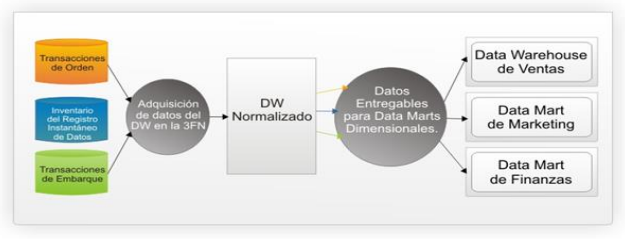
\includegraphics[width=15cm]{./IMAGENES/imgleydi2}
				\end{center}
			\end{figure}

La arquitectura que plantea Bill Inmon consta de las siguientes partes: 
\begin{itemize}
		\item Fuente de la Información: Inicia el proceso de creación de un DW, conociendo la información que se necesita de todas las herramientas de las que se tengan acceso, ir a las necesidades de información que se necesitan con la finalidad de un resultado para crear un DW.

		\item Data Warehouse: La necesidad de normalizar toda la información extraída para ser almacenada en un DW, los cuales serán procesados y consultados por un DM.
		\item Data Marts: Se crean un subconjunto de los datos de un DW con el objetivo de responder a un determinado análisis o necesidad de una población, de un departamento en específico.
		\item Explotación de los datos: Se refiere a la manera de presentación de la información para ser consultada y analizada por las áreas. En cuanto a la arquitectura interna de un DW, Bill Inmon considera las siguientes características:

			\begin{itemize}
				\item Normalización: el DW debe ser basado y diseñado, conforme al diseño de las bases de datos transaccionales con las que se esté interactuando.
				\item Tercera Forma normal: la prioridad es que el modelo de datos esté construido en TFN con lo cual se tenga mayor relación entre los objetos de la base de datos.
			\end{itemize}

\end{itemize}
\subsection{La estructura del DataWarehouse}	
En cuanto a la estructura interna del DataWarehouse, para Inmon la prioridad es que el modelo de datos esté construido en tercera forma normal. Por dar una breve explicación de lo que esto significa, el proceso de normalización consiste en aplicar una serie de reglas o normas a la hora de establecer las relaciones entre los diferentes objetos dentro de la base de datos. Con este proceso de normalización se consiguen muchos beneficios, como evitar la redundancia de los datos, mantener su integridad referencial, facilitar el mantenimiento de las tablas y disminuir el tamaño de la base de datos. Sin embargo, a diferencia de los DataWarehouse desnormalizados, las consultas exigen el empleo de queries mucho más complejas, lo que dificulta el análisis directo de la información y el uso de las herramientas de reporting. De ahí, la necesidad de construir los DataMarts que, como ya comenté, están basados en modelos dimensionales de estrella o copo de nieve, diseños fácilmente explotables por estas herramientas de análisis de datos.

			\begin{figure}[htb]
				\begin{center}
					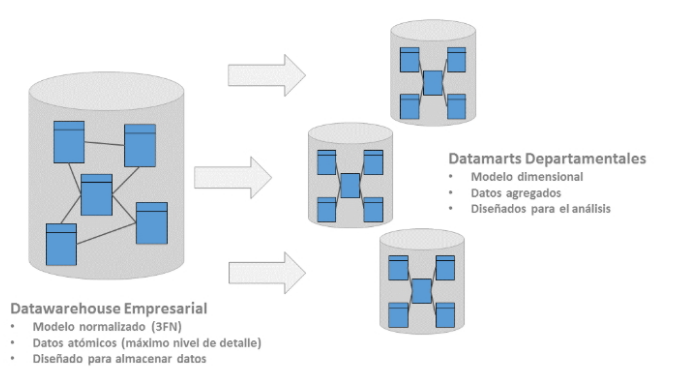
\includegraphics[width=15cm]{./IMAGENES/imgleydi3}
				\end{center}
			\end{figure}
	%%
	%\linenumbers
	
	%% main text

\subsection{METODOLOGIA SEGUN KIMBALL}	


La Metodología Kimball, es una metodología empleada para la construcción de un almacén de datos (data warehouse, DW) que no es mas que, una colección de datos orientada a un determinado ámbito (empresa, organización, etc.), integrado, no volátil y variable en el tiempo, que ayuda a la toma de decisiones en la entidad en la que se utiliza.

La metodología de Kimball, llamada Modelo Dimensional (Dimensional Modeling), se basa en lo que se denomina Ciclo de Vida Dimensional del Negocio (Business Dimensional Lifecycle). Esta metodología es considerada una de las técnicas favoritas a la hora de construir un Data Warehouse.
Ralf Kimball (1944) es considerado el inventor del Modelo Dimensional y pionero en Data Warehouse y Inteligencia de Negocios. Define un almacén de datos como: "una copia de las transacciones de datos específicamente estructurada para la consulta y el análisis". También fue Kimball quien determinó que un data warehouse no era más que: "la unión de todos los Data Marts de una entidad".
En el Modelo Dimensional se constituyen modelos de tablas y relaciones con el propósito de optimizar la toma de decisiones, con base en las consultas hechas en una base de datos relacional que están ligadas con la medición o un conjunto de mediciones de los resultados de los procesos de negocio.

			\begin{itemize}
				\item Enfoque Kimball:
				\end{itemize}

				
			\begin{figure}[htb]
				\begin{center}
					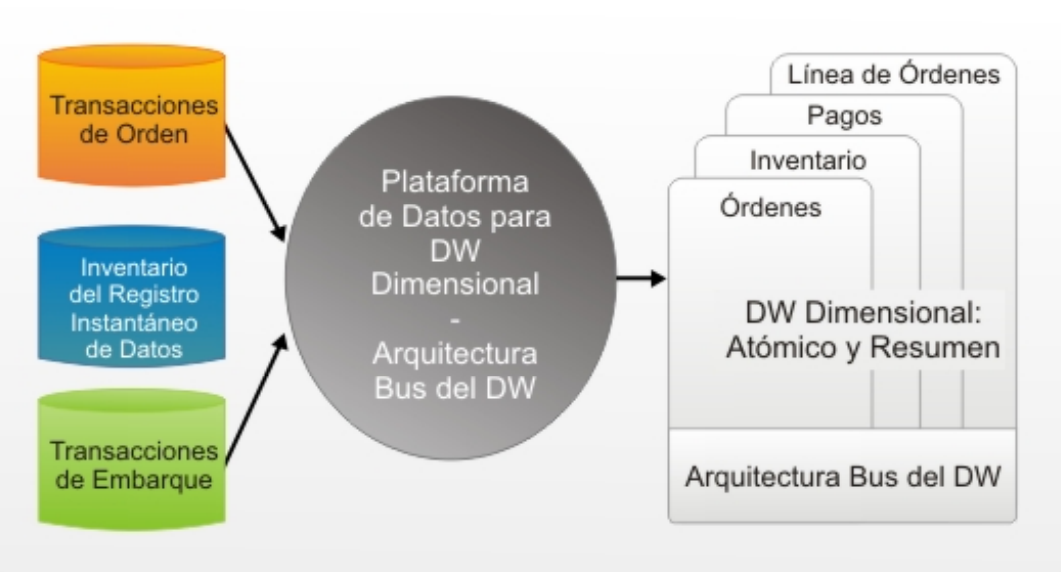
\includegraphics[width=15cm]{./IMAGENES/kimball1}
				\end{center}
			\end{figure}
				
			\begin{itemize}

				\item Objetivo:
				
				El Modelo Dimensional es una técnica de diseño lógico que tiene como objetivo presentar los datos dentro de un marco de trabajo estándar e intuitivo, para permitir su acceso con un alto rendimiento. Cada Modelo Dimensional esta compuesta por una tabla con una llave combinada, llamada tabla de hechos, y con un conjunto de tablas más pequeñas llamadas tablas de dimensiones. Los elementos de estas tablas se pueden definir de la siguiente manera:
				
			
\end{itemize}


			\begin{itemize}
				\item Hechos: es una colección de piezas de datos y datos de contexto. Cada hecho representa una parte del negocio, una transacción o un evento.
				\item Dimensiones: es una colección de miembros, unidades o individuos del mismo tipo.
				\item Medidas: son atributos numéricos de un hecho que representan el comportamiento del negocio relativo a una dimensión.
				
				Cada punto de entrada a la tabla de hechos esta conectado esta conectado a una dimensión, lo que permite determinar el contexto de los hechos.\\
Una base de datos dimensional se puede concebir como un cubo de tres o cuatro dimensiones (OLAP), en el que los usuarios pueden acceder a un porción de la base de datos a lo largo de cualquiera de sus dimensiones.\\
Dado que es muy común representar a un modelo dimensional como un tabla de hechos rodeada por las tablas de dimensiones, frecuentemente se le denomina también modelo estrella o esquema de estrella-unión.\\

			\end{itemize}
			
\begin{itemize}

			\item Ciclo de Vida Kimball:
			La metodología se basa en lo que Kimball denomina Ciclo de Vida Dimensional del Negocio (Business Dimensional Lifecycle). Este ciclo de vida del proyecto de Data Warehouse, está basado en cuatro principios básicos: \\
•	Centrarse en el negocio: Hay que concentrarse en la identificación de los requerimientos del negocio y su valor asociado, y usar estos esfuerzos para desarrollar relaciones sólidas con el negocio, agudizando el análisis del mismo y la competencia consultiva de los implementadores. \\
•	Construir una infraestructura de información adecuada: Diseñar una base de información única, integrada, fácil de usar, de alto rendimiento donde se reflejará la amplia gama de requerimientos de negocio identificados en la empresa. \\
•	Realizar entregas en incrementos significativos: Crear el almacén de datos (DW) en incrementos entregables en plazos de 6 a 12 meses. Hay que usar el valor de negocio de cada elemento identificado para determinar el orden de aplicación de los incrementos. En esto la metodología se parece a las metodologías ágiles de construcción de software. \\
•	Ofrecer la solución completa: Proporcionar todos los elementos necesarios para entregar valor a los usuarios de negocios. Para comenzar, esto significa tener un almacén de datos sólido, bien diseñado, con calidad probada, y accesible. También se deberá entregar herramientas de consulta ad hoc, aplicaciones para informes y análisis avanzado, capacitación, soporte, sitio web y documentación.

			\end{itemize}


			\begin{figure}[htb]
				\begin{center}
					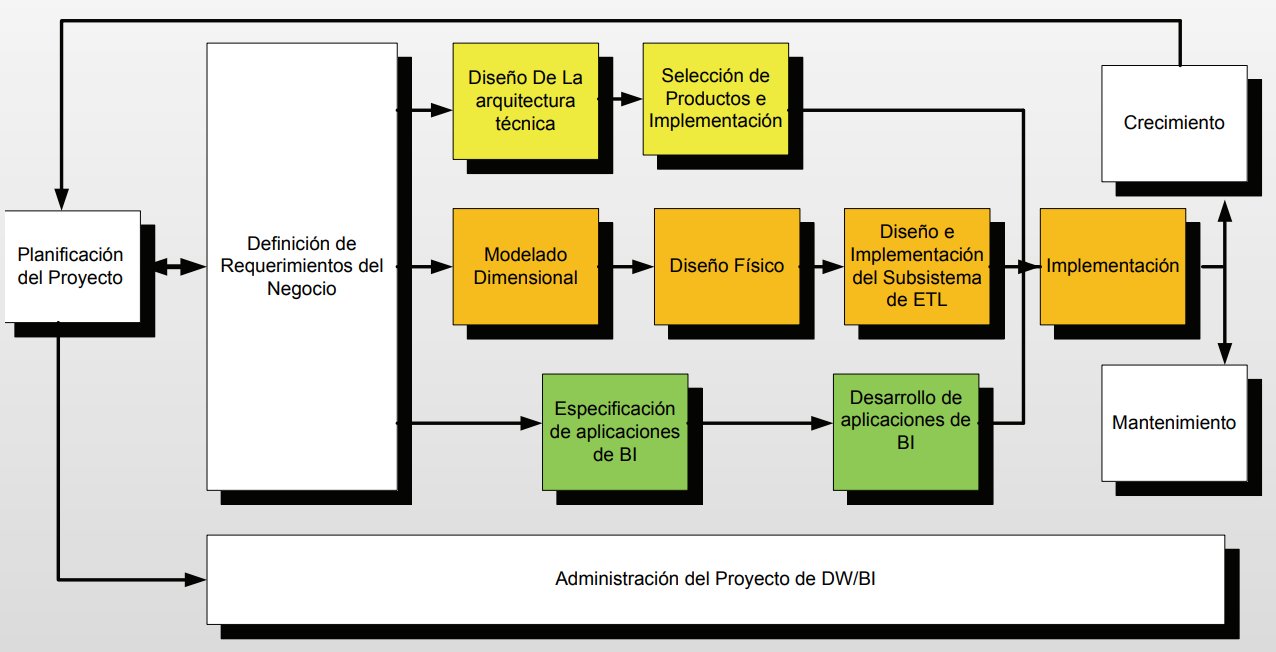
\includegraphics[width=15cm]{./IMAGENES/kimball2}
				\end{center}
			\end{figure}

Como se muestra en la figura, los Requerimientos del Negocio son el soporte inicial de las tareas subsiguientes. También tiene influencia en el plan de proyecto (puede notar la doble fecha entre la caja de definición de requerimientos y la de planificación).\\

Podemos también ver tres rutas o caminos que se enfocan en tres diferentes áreas:\\

•	Tecnología (Camino Superior): Implica tareas relacionadas con  software específico, por ejemplo, Microsoft SQL Analysis Services. \\
•	Datos (Camino del medio): En la misma diseñaremos e  implementaremos el modelo dimensional, y desarrollaremos el  subsistema de Extracción, Transformación y Carga (Extract,  Transformation, and Load - ETL) para cargar el DW. \\
•	Aplicaciones de Inteligencia de Negocios (Camino Inferior): En  esta ruta se encuentran tareas en las que diseñamos y  desarrollamos las aplicaciones de negocios para los usuarios  finales. \\

Estas rutas se combinan cuando se instala finalmente el sistema. Se observa la actividad general de administración del proyecto. Describiendo cada una de las tareas:\\

			\begin{itemize}

				\item PLANIFICACIÓN:
				
				En este proceso se determina el propósito del proyecto de DW/BI, sus objetivos específicos y el alcance de este, los principales riesgos y una aproximación inicial a las necesidades de información.

En la visión de programas y proyectos de Kimball, Proyecto, se refiere a una iteración simple del Ciclo de Vida de Kimball, desde el lanzamiento hasta el despliegue.

 Esta tarea incluye las siguientes acciones típicas de un plan de proyecto:
- Definir el alcance (Entender los Requerimientos del Negocio)
- Identificar las tareas
- Programar las tareas
- Planificar el uso de los recursos
- Asignar la carga de trabajo a los recursos
- Elaboración de un documento final que representa un plan del proyecto

Busca identificar la definición y el alcance que tiene el proyecto de DWH. Esta etapa se concentra sobre la definición del proyecto, donde, a nivel de planificación, se establece la identidad del mismo, el personal, desarrollo del plan de proyecto, el seguimiento y la monitorización.


				\item ANÁLISIS DE REQUERIMIENTOS: 
				
				 La definición de los requerimientos es en gran medida un proceso de entrevistar al personal de negocio y técnico, pero siempre conviene tener un poco de preparación previa. Se debe aprender tanto como se pueda sobre el negocio, los competidores, la industria y los clientes del mismo. Hay que leer todos los informes posibles de la organización; rastrear los documentos de estrategia interna; entrevistar a los empleados, analizar lo que se dice en la prensa acerca de la organización, la competencia y la industria. Se deben conocer los términos y la terminología del negocio.

Es un factor determinante en el éxito de un proceso de DWH. Los diseñadores de los Data Warehouse deben tener en claro cuales son los factores claves que guían el negocio para determinar efectivamente los requerimientos y traducirlos en consideraciones de diseño apropiadas.

				\item MODELADO DIMENSIONAL: 
				
				El proceso de diseño comienza con un modelo dimensional de alto nivel obtenido a partir de los procesos priorizados de la matriz descrita en el punto anterior. El proceso iterativo consiste en cuatro pasos: 

- Elegir el Proceso de Negocio.
- Establecer el Nivel de Granularidad.
- Elegir las Dimensiones.
- Identificar medidas y las tablas de hechos.
Se comienza con una matriz donde se determina la dimensionalidad de cada indicador para luego especificar los diferentes grados de detalle dentro de cada concepto del negocio.

				\item DISEÑO FÍSICO: 

Se centra en la selección de las estructuras necesarias para soportar el diseño lógico. Un elemento principal de este proceso es la definición de estándares del entorno de la base de datos. La indexación y las estrategias de particionamiento se determinan en esta etapa.

En esta parte, intentamos contestar las siguientes preguntas: 

- ¿Cómo puede determinar cuán grande será el sistema de DW\/BI? 
-¿Cuáles son los factores de uso que llevarán a una configuración más grande y más compleja? 
-¿Cómo se debe configurar el sistema?
-¿Cuánta memoria y servidores se necesitan? ¿Qué tipo de almacenamiento y procesadores? 
- ¿Cómo instalar el software en los servidores de desarrollo, prueba y producción? 
- ¿Qué necesitan instalar los diferentes miembros del equipo de DW/BI en sus estaciones de trabajo? 
- ¿Cómo convertir el modelo de datos lógico en un modelo de datos físicos en la base de datos relacional? 
- ¿Cómo conseguir un plan de indexación inicial? 
- ¿Debe usarse la partición en las tablas relacionales?


				\item DISEÑO DEL SISTEMA DE EXTRACCIÓN, TRANSFORMACIÓN Y CARGA (ETL):  \\
				
				
				Es la base sobre la cual se alimenta el Datawarehouse. Si el sistema ETL se diseña adecuadamente, puede extraer los datos de los sistemas de origen de datos, aplicar diferentes reglas para aumentar la calidad y consistencia de los mismos, consolidar la información proveniente de distintos sistemas, y finalmente cargar (grabar) la información en el DW en un formato acorde para la utilización por parte de las herramientas de análisis. \\

Tiene como principales actividades la extracción, transformación y carga (ETL). Estas actividades son altamente críticas ya que tienen que ver con la materia prima del Data Warehouse que son los datos.\\


Algunas aplicaciones analíticas comunes incluyen:

- Análisis de la eficacia de la promociones
- Análisis de rutas de acceso en un sitio Web
- Análisis de afinidad de programas
- Planificación del espacio en espacios comerciales
- Detección de fraudes
- Administración y manejo de categorías de productos


			\begin{figure}[htb]
				\begin{center}
					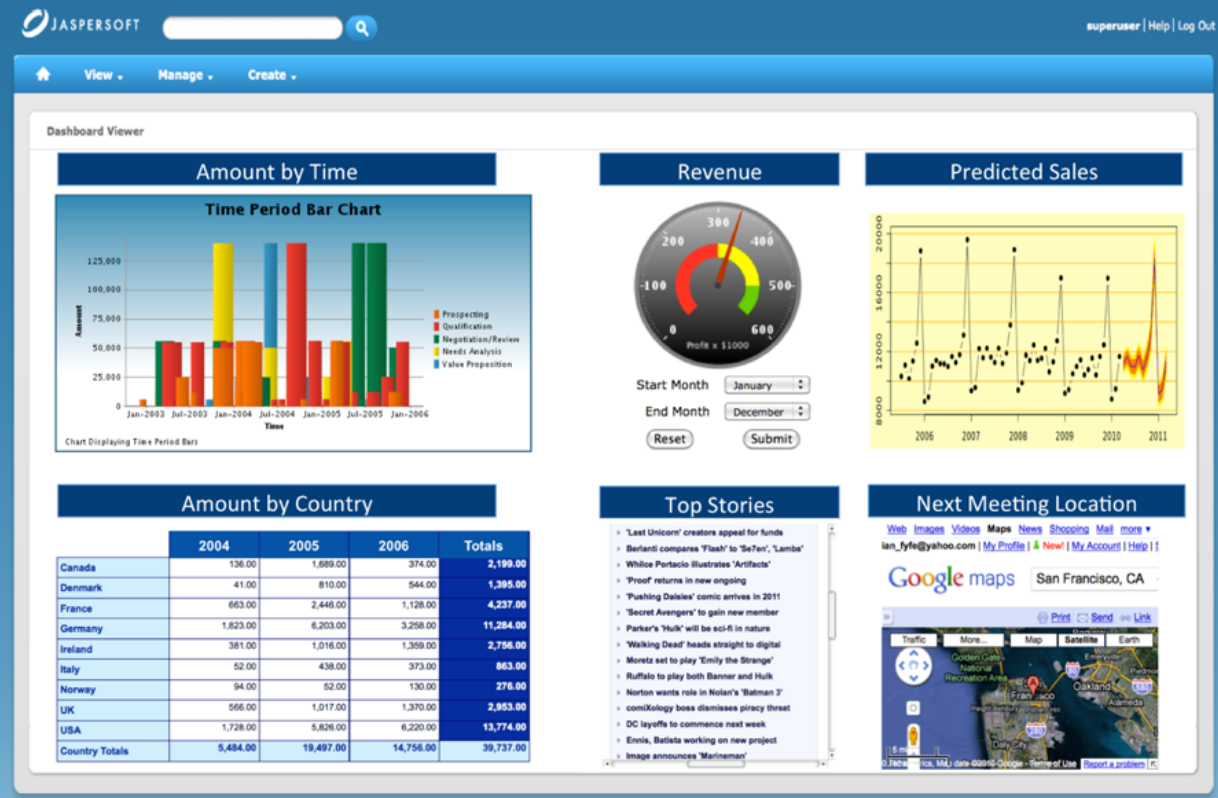
\includegraphics[width=15cm]{./IMAGENES/kimball3}
				\end{center}
			\end{figure}
			
			\begin{figure}[htb]
				\begin{center}
					
\includegraphics[width=15cm]{./IMAGENES/kimball4}
				\end{center}
			\end{figure}

				
				\item ESPECIFICACIÓN Y DESARROLLO DE APLICACIONES BI:  \\

Las aplicaciones de BI son la cara visible de la inteligencia de negocios: los informes y aplicaciones de análisis proporcionan información útil a los usuarios. Las aplicaciones de BI incluyen un amplio espectro de tipos de informes y herramientas de análisis, que van desde informes simples de formato fijo a sofisticadas aplicaciones analíticas que usan complejos algoritmos e información del dominio. Kimball divide a estas aplicaciones en dos categorías basadas en el nivel de sofisticación, y les llama informes estándar y aplicaciones analíticas.\\

En esta fase se deben tener en cuenta tres factores: los requerimientos de negocio, los actuales entornos técnicos, y las directrices técnicas y estratégicas futuras planificadas por la compañía, lo que permitirá establecer el diseño de la arquitectura técnica del entorno del Data Warehouse.\\

Diseño:\\

- Identifica las aplicaciones de BI candidatas y interfaces de navegación.\\
- Orienta las necesidades de los usuarios.\\

Desarrollo:\\

- Configuración de los metadatos del negocio.\\
- Construcción y validación de aplicaciones\\

			\end{itemize}




\subsection{COMPARACION DE METODOLOGIAS}	
El datawarehouse de Kimball está orientado a la consulta de la información, por lo que su estructura interna está especialmente diseñada para garantizar una explotación de los datos rápida y sencilla, no requiriendo usuarios especializados para ello. Por el contrario, el datawarehouse de Inmon persigue la integración de todos los datos de la compañía, estando orientado hacia el almacenaje de grandes volúmenes de datos, por lo que su estructura interna normalizada se diseña para evitar la redundancia de datos, simplificar las labores de mantenimiento, etc. cuestiones que complican las consultas de la información, requiriendo que los usuarios finales estén mucho más especializados.


			\begin{figure}[htb]
				\begin{center}
					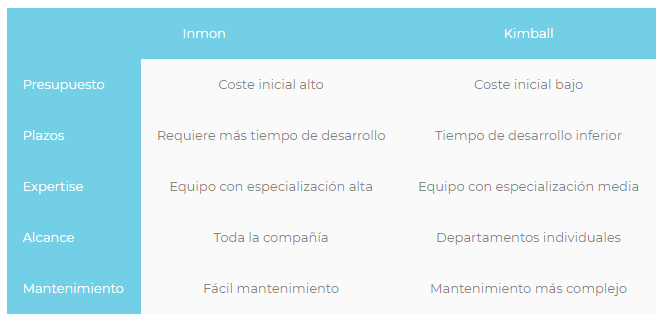
\includegraphics[width=15cm]{./IMAGENES/imgleydi4}
				\end{center}
			\end{figure}

Así, podríamos decir que el enfoque de Kimball se ajusta más a proyectos pequeños en los que se persiga un sistema fácilmente explotable y entendible por el usuario y de rápido desarrollo, siendo el modelo de Inmon más apropiado para sistemas complejos de mayor envergadura.
Todo proyecto tiene sus propias peculiaridades, siendo cada caso único e independiente, por lo que resulta necesario llevar a cabo un estudio de todas ellas antes de decantarnos por una solución u otra, de forma que podamos hacernos una idea sobre qué modelo se ajusta mejor a las condiciones de nuestro proyecto.



%%
	
	%%
	%\linenumbers
	
	%% main text
\section{Conclusion}
\begin{itemize}
\item Conclusion 1 : \\
La metodología de Kimball proporciona una base empírica y
metodológica adecuada para las implementaciones de almacenes de
datos pequeños y medianos, dada su gran versatilidad y su enfoque
ascendente, que permite construir los almacenes en forma escalonada.
Además presenta una serie de herramientas, tales como planillas,
gráficos y documentos, que proporcionan una gran ayuda para iniciarse
en el ámbito de la construcción de un Datawarehouse. 
\item Conclusion 2 : \\
Inmon usa los almacenes de datos como separación física del almacén de datos de la empresa y están diseñados para usos departamentales. Mientras que en la arquitectura de Kimball, no es necesario separar los mercados de datos del almacén de datos dimensional.
\item Conclusion 3 : \\
La metodología de Kimball es ideal para los primeros pasos de implantación de BI a un cliente, cuando la complejidad de almacenamiento de datos no es demasiado grande y donde la infraestructura del BI se encarga de los datos procedentes de un número limitado de fuentes. Sin embargo, cuando el almacén de datos adquiere complejidad, entonces es peligroso forzar el desarrollo de esta metodología. En el mundo del BI, cuando las cosas adquieren gran complejidad, es el momento de introducir nuevos enfoques al problema, como el propuesto por Inmon.


\end{itemize}

	\newpage
	
	\bibliographystyle{apalike} 	%ESTILO
	\bibliography{BIBLIOGRAFIA}	 
	\citep{silva2017gestion}  
	%\citep{trimi2012business}
	%\citep{rytkonen2014business}
\citep{rivadera2010metodologia}  
\citep{leonard2013metodologias}

\end{document}

